\chapter{METODE PENELITIAN}\label{cha:metode}


\section{Waktu dan Tempat Pelaksanaan Penelitian}
\paragraph{}Penelitian ini direncanakan untuk dilaksanakan secara intensif selama bulan Februari, memanfaatkan momentum awal tahun untuk mencapai hasil yang optimal. Lokasi penelitian berada di \textbf{Jalan Desa Cipadung, Gang Bho Optikal, RT 03 RW 04, Kosan Armani Nomor 104}. Lokasi ini dapat dengan mudah ditemukan karena terdapat pos ronda di area Gang Bho, wilayah Cibiru, Kota Bandung, Jawa Barat, dengan kode pos 40614.

\paragraph{}Keunikan penelitian ini terletak pada penggunaan alat yang dirancang secara khusus dengan tingkat presisi tinggi untuk mendukung seluruh tahap eksperimen. Dengan lokasi strategis dan penggunaan alat inovatif, penelitian ini diharapkan dapat memberikan kontribusi yang signifikan.

\begin{figure}
    \centering
    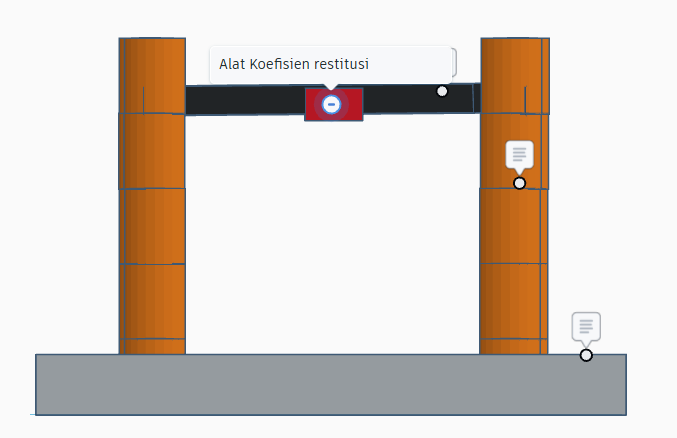
\includegraphics[width = 18pc]{images/Ilustrasi Alat.png}
    \caption{Ilustrasi Alat}
    \label{fig:ilustrasi_alat}
\end{figure}
\paragraph{}Skema berikut menunjukkan alat yang dilengkapi dengan tiang penyangga dan tiang penopang pada box alat penelitian, yang dirancang untuk mencegah goncangan dan memastikan kestabilan selama proses pengambilan data.
\begin{figure}
    \centering
    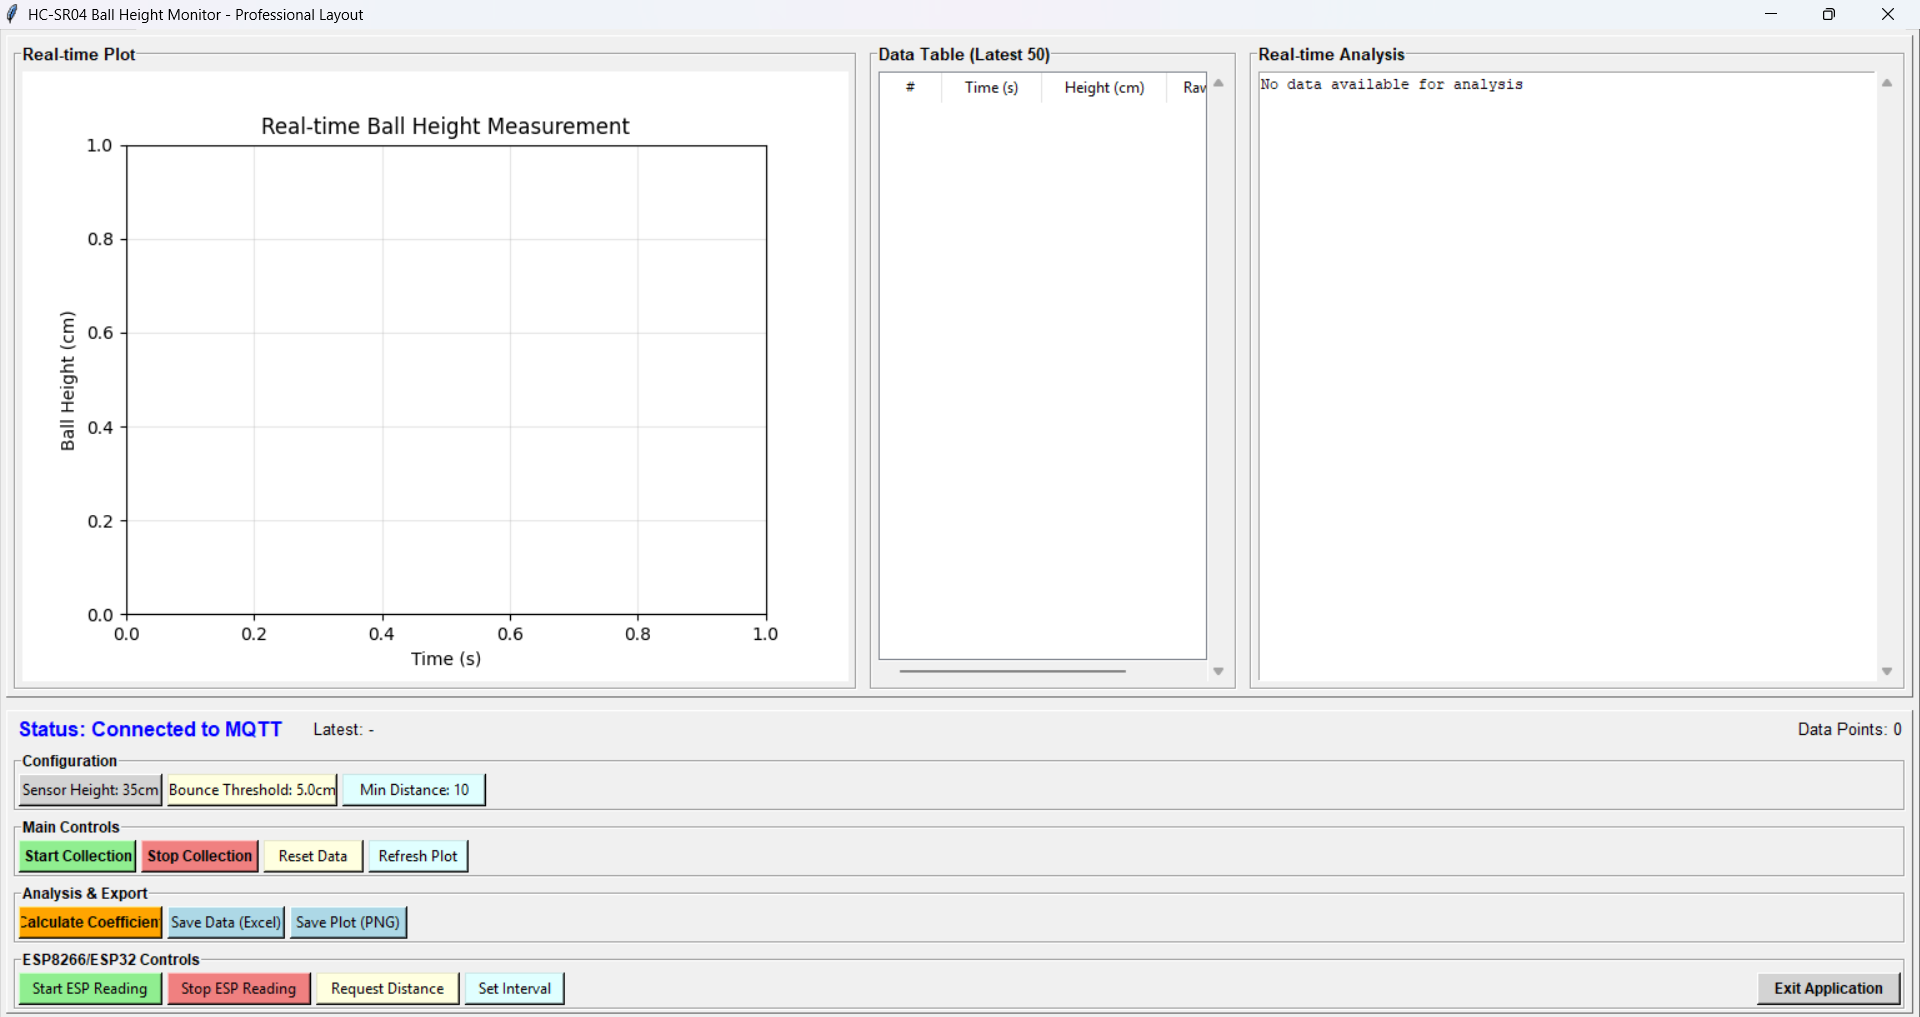
\includegraphics[width =\textwidth]{images/Tampilan GUI.png}
    \caption{Tampilan GUI}
    \label{fig:tampilan_gui}
\end{figure}
\paragraph{}Desain antarmuka pengguna aplikasi Python ini menerapkan prinsip Human-Computer Interaction (HCI) modern dengan mengintegrasikan teknologi Internet of Things (IoT) berbasis protokol Message Queuing Telemetry Transport (MQTT) untuk monitoring koefisien restitusi secara real-time. Implementasi graphical user interface (GUI) menggunakan framework Tkinter menyediakan dashboard interaktif yang memungkinkan operator melakukan kontrol sistem sensor, visualisasi data time-series, dan analisis statistik dengan tingkat responsivitas tinggi. Arsitektur client-server ini memanfaatkan cloud broker HiveMQ sebagai middleware komunikasi yang menjamin delivery reliability dan scalability sistem monitoring jarak jauh.

\paragraph{}Interface aplikasi dirancang dengan modular architecture yang terdiri dari control panel untuk command transmission, real-time plotting module untuk visualization data trajectory bola, dan analysis dashboard untuk statistical computation koefisien restitusi. Setiap komponen GUI terintegrasi dengan event-driven programming model yang memastikan seamless interaction antara user input dan system response. Protokol MQTT Quality of Service (QoS) level 1 diimplementasikan untuk guaranteed message delivery antara aplikasi Python dan embedded device ESP8266, sedangkan JSON serialization digunakan untuk structured data exchange yang mempertahankan data integrity dan parsing efficiency.
\begin{figure}
    \centering
    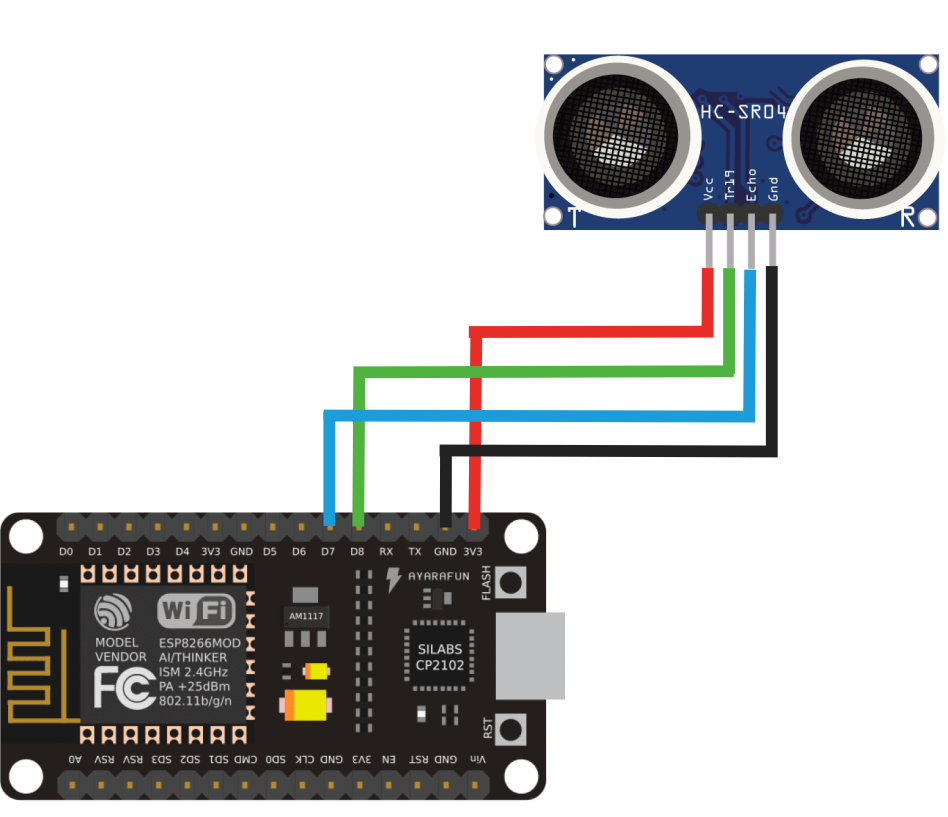
\includegraphics[width=0.5\linewidth]{images/Skematik Rangkaian.png}
    \caption{skematik rangkaian}
    \label{fig:skematik_rangkaian}
\end{figure}
\paragraph{}Ini adalah skematik rangkaian yang menunjukkan cara menghubungkan sensor HCSR-04 dengan modul ESP8266. Pada rangkaian ini, VCC dari HCSR-04 disambungkan ke pin 3V pada ESP8266, sedangkan GND HCSR-04 dihubungkan ke GND ESP8266. Untuk pin TRIG, HCSR-04 dapat disambungkan ke pin mana saja pada ESP8266, namun dalam contoh ini digunakan pin D8. Begitu juga dengan pin ECHO, yang disambungkan ke pin D7, meskipun dapat disesuaikan dengan pin lain sesuai kebutuhan.
\paragraph{}Eksperimen dilakukan sebanyak 100 kali dengan menggunakan lima jenis bola yang berbeda. Setiap jenis bola diuji sebanyak 20 kali.

\section{Alat dan Bahan Penelitian}
Alat dan bahan yang digunakan dalam penelitian ini dijelaskan sebagai berikut:

\subsection{Alat Penelitian}
Berikut adalah daftar alat yang digunakan:
\begin{table}[H]
\caption{Tabel Peralatan}
\label{tab:alat}
\begin{center}
    \begin{tabular}{|l|l|l|}
    \hline
        \textbf{No} & \textbf{Alat Penelitian} & \textbf{Jumlah Alat} \\\hline
        1 & Laptop & 1 buah \\\hline
        2 & ESP8266 & 1 buah \\\hline
        3 & HCSR-04 & 1 buah \\\hline
        4 & Kabel Jumper & Secukupnya \\\hline
        5 & Akrilik & Secukupnya \\\hline
        6 & Pipa Besi & Secukupnya \\\hline
        7 & Mur dan Baut & Secukupnya \\\hline
        8 & Penyambung Pipa & Secukupnya \\\hline
        9 & \textit{Software} Arduino & - \\\hline
    \end{tabular}
\end{center}
\end{table}

\subsection{Bahan Penelitian}
Berikut adalah daftar bahan yang digunakan:
\begin{table}[H]
\caption{Tabel Bahan}
\label{tab:bahan}
\begin{center}
    \begin{tabular}{|l|l|l|}
    \hline
        \textbf{No} & \textbf{Bahan Penelitian} & \textbf{Jumlah Bahan} \\\hline
        1 & Bola Tenis Meja & 1 buah \\\hline
        2 & Bola Bekel & 1 buah \\\hline
        3 & Bola Sepak Karet & 1 buah \\\hline
        4 & Bola Plastik & 1 buah \\\hline
        5 & Bola Tenis lapang & 1 buah \\\hline
    \end{tabular}
\end{center}
\end{table}

\section{Diagram Alir Penelitian}
\subsection{Flowchart Program Python}

\begin{figure}[H]
\centering
\begin{tikzpicture} [
    node distance=0.5cm,
    start/.style={ellipse, draw=black, thick, fill=green!30, minimum width=2.5cm, minimum height=1cm, font=\tiny, text centered},
    process/.style={rectangle, draw=black, thick, fill=blue!30, minimum width=2.5cm, minimum height=1cm, font=\tiny, text centered},
    decision/.style={diamond, draw=black, thick, fill=yellow!30, minimum width=2cm, minimum height=2cm, font=\tiny, text centered, inner sep=1pt},
    terminal/.style={ellipse, draw=black, thick, fill=red!30, minimum width=2cm, minimum height=1cm, font=\tiny, text centered},
    arrow/.style={->, thick, >=stealth}
]

% Layer 1: Define all nodes first (foreground)
\node[start] (start) {Mulai\\Aplikasi Python};
\node[process, below=of start] (init) {Inisialisasi GUI\\Setup MQTT\\Koneksi Broker};
\node[process, below=of init] (loop) {Loop Event Utama};
\node[decision, below=of loop, xshift=-3cm] (mqtt_msg) {Pesan\\MQTT?};
\node[decision, below=of loop, xshift=3cm] (user_action) {Aksi\\Pengguna?};
\node[process, below=of mqtt_msg] (parse) {Parse JSON\\Validasi Data};
\node[decision, below=of parse] (collecting) {Mengumpulkan\\Data?};
\node[process, below=of collecting] (store) {Simpan Data\\Update Plot};
\node[process, below=of user_action] (handle) {Tangani Input\\Pengguna};
\node[decision, below=of handle] (analyze) {Hitung\\Koefisien?};
\node[process, below=of analyze] (calc) {Deteksi Pantulan\\Hitung e};
\node[process, below=of store, xshift=3cm] (update) {Update GUI\\Tampilkan Hasil};
\node[terminal, below=of update] (end) {Keluar\\Aplikasi};

% Layer 2: Draw all arrows in background
\begin{scope}[on background layer]
    % Main Flow Arrows
    \draw[arrow, blue!70, line width=1.2pt] (start) -- (init);
    \draw[arrow, blue!70, line width=1.2pt] (init) -- (loop);
    
    % Branch to decisions
    \draw[arrow, blue!70, line width=1.2pt] (loop) -- (mqtt_msg);
    \draw[arrow, blue!70, line width=1.2pt] (loop) -- (user_action);
    
    % MQTT Branch
    \draw[arrow, green!70, line width=1.2pt] (mqtt_msg) -- node[right, fill=white, inner sep=1pt, font=\tiny] {Ya} (parse);
    \draw[arrow, green!70, line width=1.2pt] (parse) -- (collecting);
    \draw[arrow, green!70, line width=1.2pt] (collecting) -- node[right, fill=white, inner sep=1pt, font=\tiny] {Ya} (store);
    \draw[arrow, green!70, line width=1.2pt] (store) -- (update);
    
    % User Branch
    \draw[arrow, purple!70, line width=1.2pt] (user_action) -- node[left, fill=white, inner sep=1pt, font=\tiny] {Ya} (handle);
    \draw[arrow, purple!70, line width=1.2pt] (handle) -- (analyze);
    \draw[arrow, purple!70, line width=1.2pt] (analyze) -- node[right, fill=white, inner sep=1pt, font=\tiny] {Ya} (calc);
    \draw[arrow, purple!70, line width=1.2pt] (calc) -- (update);
    
    % No Branches to Update
    \draw[arrow, red!60, line width=1pt] (mqtt_msg) -- node[above, fill=white, inner sep=1pt, font=\tiny] {Tidak} ++(3,0) |- (update);
    \draw[arrow, red!60, line width=1pt] (user_action) -- node[above, fill=white, inner sep=1pt, font=\tiny] {Tidak} ++(-3,0) |- (update);
    \draw[arrow, red!60, line width=1pt] (collecting) -- node[left, fill=white, inner sep=1pt, font=\tiny] {Tidak} ++(-1.5,0) |- (update);
    \draw[arrow, red!60, line width=1pt] (analyze) -- node[left, fill=white, inner sep=1pt, font=\tiny] {Tidak} ++(-1.5,0) |- (update);
    
    % Loop Back
    \draw[arrow, orange!60, line width=1pt, dashed] (update) -- ++(4,0) |- (loop);
    
    % Exit
    \draw[arrow, gray!70, line width=1.2pt] (update) -- (end);
\end{scope}

\end{tikzpicture}
\caption{Flowchart Program Python}
\end{figure}

\textbf{Penjelasan Program Python:} 

Aplikasi Python ini adalah program utama yang berfungsi sebagai pusat kontrol seluruh sistem monitoring koefisien restitusi bola. Program ini dirancang dengan antarmuka grafis (GUI) yang user-friendly menggunakan library Tkinter sehingga pengguna dapat dengan mudah mengoperasikan sistem tanpa perlu memahami kode programming.

\textbf{Cara Kerja Program Python:}

\paragraph{Inisialisasi Sistem} Saat program dimulai, sistem melakukan setup GUI (tampilan aplikasi), mengatur koneksi MQTT ke cloud broker HiveMQ, dan mempersiapkan semua komponen yang diperlukan untuk monitoring real-time. Proses ini memastikan bahwa semua library yang diperlukan telah dimuat dengan benar dan interface pengguna siap untuk digunakan.

\paragraph{Loop Utama Monitoring} Program masuk ke dalam loop pemantauan kontinyu yang secara bersamaan memantau dua hal: (a) pesan data sensor yang dikirim ESP8266 melalui internet via MQTT, dan (b) interaksi pengguna seperti klik tombol atau pengaturan parameter. Loop ini berjalan secara terus-menerus untuk memastikan responsivitas sistem terhadap input dan data yang masuk.

\paragraph{Penerimaan Data Sensor} Ketika ESP8266 mengirim data jarak dalam format JSON melalui internet, program Python menerima, memvalidasi, dan mengonversi data jarak menjadi tinggi bola dengan rumus: tinggi\_bola = tinggi\_sensor - jarak\_terukur. Validasi data dilakukan untuk memastikan kualitas pengukuran dan menghilangkan noise atau error yang mungkin terjadi.

\paragraph{Penyimpanan dan Visualisasi} Data yang valid disimpan dalam array waktu dan tinggi, kemudian divisualisasikan secara real-time dalam grafik yang terus ter-update untuk memudahkan observasi pergerakan bola. Sistem visualisasi ini memungkinkan operator untuk melihat pola pantulan bola secara langsung dan mendeteksi anomali dalam pengukuran.

\paragraph{Analisis Otomatis} Sistem menggunakan algoritma deteksi puncak untuk mengidentifikasi titik-titik pantulan bola, menghitung koefisien restitusi dengan rumus fisika $e = \sqrt{h_2/h_1}$, dan menghasilkan laporan komprehensif tentang karakteristik elastisitas bola. Analisis ini dilakukan secara otomatis setelah cukup data terkumpul untuk memastikan akurasi hasil perhitungan.

\newpage

\subsection{Flowchart Program ESP8266}

\begin{figure}[H]
\centering
\begin{tikzpicture} [
    node distance=0.5cm,
    start/.style={ellipse, draw=black, thick, fill=green!30, minimum width=2.5cm, minimum height=1cm, font=\tiny, text centered},
    process/.style={rectangle, draw=black, thick, fill=blue!30, minimum width=2.5cm, minimum height=1cm, font=\tiny, text centered},
    decision/.style={diamond, draw=black, thick, fill=yellow!30, minimum width=2cm, minimum height=2cm, font=\tiny, text centered, inner sep=1pt},
    arrow/.style={->, thick, >=stealth}
]

% Layer 1: Define all nodes first (foreground)
\node[start] (start) {Mulai\\ESP8266};
\node[process, below=of start] (init_hw) {Inisialisasi\\Pin \& Serial};
\node[process, below=of init_hw] (wifi) {Koneksi\\WiFi};
\node[process, below=of wifi] (mqtt) {Koneksi MQTT\\Subscribe Topik};
\node[process, below=of mqtt] (main_loop) {Loop Utama};
\node[decision, below=of main_loop, xshift=-3cm] (cmd_check) {Perintah\\Diterima?};
\node[decision, below=of main_loop, xshift=3cm] (read_check) {Mode Baca \&\\Interval?};
\node[process, below=of cmd_check] (parse_cmd) {Parse\\Perintah};
\node[decision, below=of parse_cmd] (cmd_type) {Jenis\\Perintah?};
\node[process, below=of cmd_type, xshift=-2cm] (start_read) {Set Pembacaan\\AKTIF};
\node[process, below=of cmd_type, xshift=2cm] (stop_read) {Set Pembacaan\\NONAKTIF};
\node[process, below=of read_check] (sensor) {Baca\\HC-SR04};
\node[process, below=of sensor] (validate) {Validasi\\Data};
\node[process, below=of validate] (json) {Buat\\JSON};
\node[process, below=of json] (publish) {Publish\\MQTT};

% Layer 2: Draw all arrows in background
\begin{scope}[on background layer]
    % Main Flow
    \draw[arrow, blue!70, line width=1.2pt] (start) -- (init_hw);
    \draw[arrow, blue!70, line width=1.2pt] (init_hw) -- (wifi);
    \draw[arrow, blue!70, line width=1.2pt] (wifi) -- (mqtt);
    \draw[arrow, blue!70, line width=1.2pt] (mqtt) -- (main_loop);
    
    % Branches
    \draw[arrow, blue!70, line width=1.2pt] (main_loop) -- (cmd_check);
    \draw[arrow, blue!70, line width=1.2pt] (main_loop) -- (read_check);
    
    % Command Flow
    \draw[arrow, green!70, line width=1.2pt] (cmd_check) -- node[right, fill=white, inner sep=1pt, font=\tiny] {Ya} (parse_cmd);
    \draw[arrow, green!70, line width=1.2pt] (parse_cmd) -- (cmd_type);
    \draw[arrow, green!70, line width=1.2pt] (cmd_type) -- node[above left, fill=white, inner sep=1pt, font=\tiny] {MULAI} (start_read);
    \draw[arrow, green!70, line width=1.2pt] (cmd_type) -- node[above right, fill=white, inner sep=1pt, font=\tiny] {BERHENTI} (stop_read);
    
    % Sensor Flow
    \draw[arrow, purple!70, line width=1.2pt] (read_check) -- node[left, fill=white, inner sep=1pt, font=\tiny] {Ya} (sensor);
    \draw[arrow, purple!70, line width=1.2pt] (sensor) -- (validate);
    \draw[arrow, purple!70, line width=1.2pt] (validate) -- (json);
    \draw[arrow, purple!70, line width=1.2pt] (json) -- (publish);
    
    % Loop Back
    \draw[arrow, orange!60, line width=1pt, dashed] (start_read) |- ++(0,-1) -| (main_loop);
    \draw[arrow, orange!60, line width=1pt, dashed] (stop_read) |- ++(0,-1) -| (main_loop);
    \draw[arrow, orange!60, line width=1pt, dashed] (publish) |- ++(-6,0) |- (main_loop);
    
    % No Action
    \draw[arrow, red!60, line width=1pt] (cmd_check) -- node[above, fill=white, inner sep=1pt, font=\tiny] {Tidak} ++(3,0) |- (main_loop);
    \draw[arrow, red!60, line width=1pt] (read_check) -- node[above, fill=white, inner sep=1pt, font=\tiny] {Tidak} ++(-3,0) |- (main_loop);
\end{scope}

\end{tikzpicture}
\caption{Flowchart Program ESP8266}
\end{figure}

\textbf{Penjelasan Program ESP8266:}

Program ESP8266 berperan sebagai sensor node cerdas yang bekerja secara autonomous (mandiri) untuk mengukur jarak menggunakan sensor ultrasonik HC-SR04 dan mengirimkan data ke aplikasi Python melalui komunikasi internet menggunakan protokol MQTT.

\textbf{Cara Kerja Program ESP8266:}

\paragraph{Inisialisasi Hardware} Saat ESP8266 dinyalakan, program melakukan setup pin GPIO untuk sensor HC-SR04 (pin trigger dan echo), mengatur komunikasi serial untuk debugging, dan menginisialisasi LED built-in sebagai indikator status. Proses ini memastikan bahwa semua komponen hardware siap digunakan dengan konfigurasi yang benar.

\paragraph{Koneksi WiFi} ESP8266 terhubung ke jaringan WiFi menggunakan SSID dan password yang telah dikonfigurasi, memungkinkan akses internet untuk komunikasi dengan broker MQTT cloud. Sistem akan mencoba koneksi berulang kali jika gagal terhubung pada percobaan pertama hingga berhasil mendapatkan koneksi yang stabil.

\paragraph{Setup MQTT} Setelah WiFi terhubung, ESP8266 melakukan koneksi ke broker MQTT di cloud (HiveMQ), subscribe ke topik command untuk menerima perintah dari Python, dan siap mempublikasikan data sensor. Konfigurasi ini memungkinkan komunikasi dua arah antara ESP8266 dan aplikasi Python melalui internet.

\paragraph{Loop Pemrosesan Command} Dalam loop utama, ESP8266 memantau perintah dari aplikasi Python seperti START\_READING (mulai pembacaan kontinyu), STOP\_READING (hentikan pembacaan), atau INTERVAL:nilai (ubah frekuensi pembacaan). Setiap perintah diproses dengan cepat untuk memastikan responsivitas sistem terhadap kontrol pengguna.

\paragraph{Pembacaan Sensor} Ketika mode pembacaan aktif, ESP8266 melakukan pengukuran jarak menggunakan HC-SR04 dengan mengirim gelombang ultrasonik dan menghitung waktu tempuh, kemudian mengkonversi ke jarak dalam satuan centimeter. Pembacaan dilakukan sesuai dengan interval yang telah ditentukan untuk menghasilkan data yang konsisten.

\paragraph{Validasi dan Pengiriman Data} Setiap hasil pembacaan divalidasi (rentang 2-400cm), dikemas dalam format JSON dengan timestamp yang direset setiap START\_READING, dan dikirim ke aplikasi Python melalui topik MQTT. Validasi ini penting untuk memastikan kualitas data dan menghindari pengiriman data yang tidak akurat atau error.

\newpage

\subsection{Komunikasi Sistem}

\textbf{Komunikasi Sistem IoT:}

Sistem ini mengimplementasikan arsitektur Internet of Things (IoT) modern berbasis protokol MQTT yang memungkinkan komunikasi real-time antara perangkat sensor (ESP8266) dan aplikasi monitoring (Python) melalui internet menggunakan cloud broker HiveMQ yang tersedia 24/7.

\textbf{Penjelasan Detail Alur Komunikasi:}

\begin{enumerate}
\item \textbf{Pengiriman Command (Python → MQTT Broker):} Aplikasi Python mengirimkan perintah kontrol seperti "START\_READING" atau "STOP\_READING" ke broker MQTT cloud melalui topik khusus "sensor/distance/cmd". Perintah ini dikirim dalam format teks sederhana yang mudah dipahami ESP8266.

\item \textbf{Penerusan Command (MQTT Broker → ESP8266):} Broker MQTT cloud secara otomatis meneruskan semua perintah yang diterima dari Python ke ESP8266 yang telah subscribe ke topik command. Proses ini terjadi dalam hitungan milidetik berkat infrastruktur cloud yang cepat.

\item \textbf{Pengiriman Data Sensor (ESP8266 → MQTT Broker):} Setelah menerima perintah START\_READING, ESP8266 mulai mengukur jarak menggunakan sensor HC-SR04 secara kontinyu dan mengirimkan data dalam format JSON ke broker MQTT melalui topik "sensor/distance". Data JSON berisi timestamp, jarak terukur, dan identitas perangkat.

\item \textbf{Penerimaan Data (MQTT Broker → Python):} Aplikasi Python yang telah subscribe ke topik data sensor menerima semua data yang dikirim ESP8266 melalui broker. Data JSON ini kemudian di-parse, divalidasi, dan dikonversi menjadi informasi tinggi bola untuk analisis real-time.
\end{enumerate}

\textbf{Keunggulan Arsitektur MQTT:}
\begin{itemize}
\item \textbf{Komunikasi Real-time:} Latensi rendah untuk monitoring langsung pergerakan bola
\item \textbf{Reliability:} Broker cloud menjamin pengiriman pesan dengan mekanisme Quality of Service (QoS)
\item \textbf{Scalability:} Dapat dengan mudah menambahkan multiple ESP8266 atau aplikasi monitoring
\item \textbf{Internet-based:} Monitoring dapat dilakukan dari jarak jauh selama ada koneksi internet
\item \textbf{Bi-directional:} Komunikasi dua arah memungkinkan kontrol penuh terhadap sistem sensor
\end{itemize}

\subsection{Spesifikasi Teknis}

\subsubsection{Format Data JSON}
\begin{itemize}
    \item \textbf{Sensor Data:} \texttt{\{"timestamp": 1.23, "distance": 25.4, \\ "device": "ESP8266\_HCSR04"\}}
    \item \textbf{Commands:} \texttt{START\_READING}, \texttt{STOP\_READING}, \texttt{INTERVAL:100}
\end{itemize}

\subsubsection{Parameter Sistem}
\begin{itemize}
    \item \textbf{Sensor Range:} 2-400 cm
    \item \textbf{Sampling Rate:} 50-5000 ms (configurable)
    \item \textbf{Analysis Formula:} $e = \sqrt{\frac{h_2}{h_1}}$
    \item \textbf{MQTT Topics:} sensor/distance, sensor/distance/cmd
\end{itemize}

\subsection{Diagram Alir untuk melakukan percobaan}

\begin{figure}[H]
\centering
\begin{tikzpicture} [
    node distance=0.5cm,
    start/.style={ellipse, draw=black, thick, fill=green!30, minimum width=2.5cm, minimum height=1cm, font=\tiny, text centered},
    process/.style={rectangle, draw=black, thick, fill=blue!30, minimum width=2.5cm, minimum height=1cm, font=\tiny, text centered},
    terminal/.style={ellipse, draw=black, thick, fill=red!30, minimum width=2cm, minimum height=1cm, font=\tiny, text centered},
    arrow/.style={->, thick, >=stealth}
]

% Define all nodes first (foreground)
\node[start] (start) {Mulai\\Percobaan};
\node[process, below=of start] (alat) {Menyiapkan Alat\\HC-SR04 \& ESP8266};
\node[process, below=of alat] (program) {Memastikan Program\\Berjalan dengan Baik};
\node[process, below=of program] (posisi) {Menempatkan Bola\\di Posisi Awal\\Dekat Sensor};
\node[process, below=of posisi] (lepas) {Melepaskan Bola\\Hingga Memantul\\pada Permukaan};
\node[process, below=of lepas] (lihat) {Melihat Hasil Data\\Pengukuran\\dari Sensor};
\node[process, below=of lihat] (simpan) {Menyimpan dan\\Mendokumentasikan\\Data yang Diperoleh};
\node[process, below=of simpan] (ulang) {Mengulangi Langkah\\Percobaan untuk\\Mendapatkan Banyak Data};
\node[terminal, below=of ulang] (end) {Selesai\\Percobaan};

% Draw all arrows in background
\begin{scope}[on background layer]
    \draw[arrow, blue!70, line width=1.2pt] (start) -- (alat);
    \draw[arrow, blue!70, line width=1.2pt] (alat) -- (program);
    \draw[arrow, blue!70, line width=1.2pt] (program) -- (posisi);
    \draw[arrow, blue!70, line width=1.2pt] (posisi) -- (lepas);
    \draw[arrow, blue!70, line width=1.2pt] (lepas) -- (lihat);
    \draw[arrow, blue!70, line width=1.2pt] (lihat) -- (simpan);
    \draw[arrow, blue!70, line width=1.2pt] (simpan) -- (ulang);
    \draw[arrow, blue!70, line width=1.2pt] (ulang) -- (end);
\end{scope}

\end{tikzpicture}
\caption{Flowchart Prosedur Percobaan}
\end{figure}

\textbf{Penjelasan Prosedur Percobaan:}

Flowchart prosedur percobaan ini menggambarkan metodologi sistematis untuk melakukan pengukuran koefisien restitusi bola menggunakan teknologi IoT modern. Setiap langkah dirancang untuk memastikan akurasi data dan reproducibility hasil eksperimen.

\subsubsection{Cara Kerja Prosedur Percobaan}

\paragraph{Persiapan Perangkat Keras} Tahap awal meliputi setup fisik sistem IoT dengan menempatkan sensor HC-SR04 pada ketinggian terukur dari lantai, menghubungkan ESP8266 ke power supply, dan memastikan semua koneksi hardware (trigger pin, echo pin, WiFi antenna) berfungsi optimal. Kalibrasi sensor dilakukan untuk memastikan pembacaan jarak yang akurat dalam rentang 2-400cm.

\paragraph{Validasi Sistem Software} Sebelum eksperimen dimulai, dilakukan pengecekan menyeluruh terhadap koneksi WiFi ESP8266, status MQTT broker connection ke HiveMQ Cloud, dan responsivitas komunikasi antara aplikasi Python dengan device sensor. Test komunikasi dilakukan dengan mengirim command sederhana dan memverifikasi response time.

\paragraph{Setup Eksperimental} Bola ditempatkan pada posisi awal yang tepat di bawah sensor HC-SR04 dengan jarak optimal (biasanya 10-30cm dari sensor) untuk memastikan deteksi yang akurat. Lingkungan eksperimen harus bebas dari interferensi suara dan getaran yang dapat mempengaruhi sensor ultrasonik.

\paragraph{Eksekusi Pengukuran} Saat bola dilepaskan, sistem mulai melakukan continuous monitoring dengan sampling rate tinggi (50-100ms interval). Data jarak real-time dikirim via MQTT dalam format JSON yang berisi timestamp presisi tinggi, nilai jarak, dan metadata perangkat untuk tracking yang akurat.

\paragraph{Real-time Data Monitoring} Operator memantau grafik real-time di aplikasi Python untuk memastikan kualitas data yang dikumpulkan. Visual feedback memungkinkan deteksi immediate terhadap anomali atau error dalam pengukuran, seperti noise berlebihan atau pembacaan yang tidak konsisten.

\paragraph{Data Persistence dan Backup} Setiap sesi pengukuran secara otomatis disimpan dalam multiple format (Excel untuk analisis statistik, JSON untuk processing lebih lanjut, dan PNG untuk dokumentasi visual). Timestamping dan naming convention yang konsisten memudahkan organization dan retrieval data.

\paragraph{Replicability dan Statistical Validity} Proses diulang multiple kali (minimum 5-10 repetisi) untuk memperoleh dataset yang statistik significant. Variasi antar-percobaan dianalisis untuk memastikan consistency dan mengidentifikasi potential systematic errors.

\paragraph{Quality Control dan Documentation} Setiap sesi percobaan didokumentasikan dengan metadata lengkap termasuk environmental conditions, ball specifications, sensor configuration, dan observation notes untuk memastikan traceability dan reproducibility eksperimen.

\newpage

\subsection{Diagram Alir untuk mengolah data}

\begin{figure}[H]
\centering
\begin{tikzpicture} [
    node distance=0.5cm,
    start/.style={ellipse, draw=black, thick, fill=green!30, minimum width=2.5cm, minimum height=1cm, font=\tiny, text centered},
    process/.style={rectangle, draw=black, thick, fill=blue!30, minimum width=2.5cm, minimum height=1cm, font=\tiny, text centered},
    terminal/.style={ellipse, draw=black, thick, fill=red!30, minimum width=2cm, minimum height=1cm, font=\tiny, text centered},
    arrow/.style={->, thick, >=stealth}
]

% Define all nodes first (foreground)
\node[start] (start) {Mulai\\Analisis Data};
\node[process, below=of start] (kumpul) {Mengumpulkan Seluruh\\Data Hasil Percobaan\\Format JSON \& Excel};
\node[process, below=of kumpul] (bersih) {Membersihkan Data\\dari Error atau\\Anomali (Filter)};
\node[process, below=of bersih] (deteksi) {Deteksi Puncak\\Pantulan dengan\\Algoritma find\_peaks};
\node[process, below=of deteksi] (hitung) {Menghitung Koefisien\\Restitusi: $e = \sqrt{h_2/h_1}$\\untuk Setiap Pantulan};
\node[process, below=of hitung] (statistik) {Menghitung Statistik:\\Rata-rata, Std Dev,\\Min, Max Koefisien};
\node[process, below=of statistik] (banding) {Membandingkan Hasil\\Antar Jenis Bola\\dan Klasifikasi Material};
\node[process, below=of banding] (laporan) {Membuat Laporan\\Lengkap dengan\\Grafik dan Analisis};
\node[terminal, below=of laporan] (end) {Selesai\\Analisis};

% Draw all arrows in background
\begin{scope}[on background layer]
    \draw[arrow, blue!70, line width=1.2pt] (start) -- (kumpul);
    \draw[arrow, blue!70, line width=1.2pt] (kumpul) -- (bersih);
    \draw[arrow, blue!70, line width=1.2pt] (bersih) -- (deteksi);
    \draw[arrow, blue!70, line width=1.2pt] (deteksi) -- (hitung);
    \draw[arrow, blue!70, line width=1.2pt] (hitung) -- (statistik);
    \draw[arrow, blue!70, line width=1.2pt] (statistik) -- (banding);
    \draw[arrow, blue!70, line width=1.2pt] (banding) -- (laporan);
    \draw[arrow, blue!70, line width=1.2pt] (laporan) -- (end);
\end{scope}

\end{tikzpicture}
\caption{Flowchart Analisis dan Pengolahan Data}
\end{figure}

\textbf{Penjelasan Proses Pengolahan Data:}

Flowchart pengolahan data menunjukkan pipeline analisis yang sophisticated untuk mengekstrak koefisien restitusi dari raw sensor data. Setiap tahap menggunakan algoritma advanced untuk memastikan akurasi dan validitas hasil analisis.

\subsubsection{Cara Kerja Pengolahan Data}


\paragraph{Data Aggregation dan Import} Sistem mengumpulkan semua file data dari multiple experiment sessions, melakukan parsing format JSON dan Excel, dan memvalidasi data integrity. Error checking dilakukan untuk mendeteksi corrupted files, missing timestamps, atau inconsistent data ranges yang dapat mempengaruhi analisis.

\paragraph{Data Preprocessing dan Noise Reduction} Raw sensor data dibersihkan menggunakan sophisticated filtering techniques termasuk low-pass Butterworth filter untuk menghilangkan high-frequency noise, outlier detection menggunakan statistical methods (IQR dan Z-score), dan data interpolation untuk mengisi missing data points yang minimal.

\paragraph{Peak Detection Algorithm} Implementasi algoritma `find\_peaks` dari SciPy dengan parameter optimization untuk mendeteksi bounce peaks yang akurat. Algorithm menggunakan multiple criteria termasuk minimum height threshold, prominence analysis, dan distance constraints untuk mengidentifikasi true bounce events sambil mengeliminasi false positives.

\paragraph{Physics-based Coefficient Calculation} Untuk setiap pasangan consecutive bounces, sistem menghitung koefisien restitusi menggunakan rumus fundamental fisika $e = \sqrt{h_2/h_1}$ dimana $h_1$ adalah tinggi bounce pertama dan $h_2$ adalah tinggi bounce kedua. Validasi dilakukan untuk memastikan $0 < e < 1$ sesuai dengan physical constraints.

\paragraph{Statistical Analysis dan Uncertainty Quantification} Comprehensive statistical analysis dilakukan termasuk calculation of mean, standard deviation, confidence intervals, dan distribution analysis. Uncertainty propagation dihitung untuk memahami error margins dan reliability dari hasil pengukuran.

\paragraph{Comparative Analysis dan Material Classification} Results dibandingkan dengan theoretical values dan empirical data dari literature untuk material classification. Machine learning algorithms dapat diimplementasikan untuk automated material identification berdasarkan bounce characteristics dan coefficient patterns.

\paragraph{Report Generation dan Visualization} Sistem menghasilkan comprehensive reports dengan high-quality visualizations termasuk time-series plots, bounce trajectory analysis, statistical distributions, dan comparison charts. Reports di-format dalam multiple outputs (PDF untuk presentation, Excel untuk further analysis, HTML untuk web sharing).

\paragraph{Data Quality Assessment dan Validation} Final stage meliputi comprehensive validation terhadap hasil analisis, consistency checking dengan physical laws, dan assessment terhadap experimental uncertainty. Quality metrics dihitung untuk mengevaluasi reliability dan accuracy dari entire measurement dan analysis process.

\section{Prosedur Penelitian}
\subsection{Pengambilan Data}
Untuk pengambilan data, alat dan bahan harus disiapkan dengan baik. Alat yang digunakan meliputi ESP8266 sebagai mikrokontroler dan modul WiFi, sensor ultrasonik HCSR-04 untuk mengukur jarak pantulan, breadboard, kabel jumper, serta sumber daya berupa baterai atau adaptor. Laptop atau PC juga diperlukan untuk pemrograman dan analisis data. Lima jenis bola yang diuji adalah bola karet, bola baseball, bola plastik, bola tenis meja, dan bola bekel. Pengujian dilakukan di ruangan dengan lantai keras dan permukaan datar guna menjaga konsistensi pantulan.

\paragraph{}Prosedur diawali dengan kalibrasi sistem. Pasang ESP8266 dan HCSR-04 menggunakan breadboard, kemudian tempatkan sensor pada ketinggian 35 cm dari lantai. Gunakan penggaris untuk memastikan pembacaan jarak oleh sensor sesuai dengan nilai sebenarnya. Program ESP8266 menggunakan perangkat lunak seperti Arduino IDE. Kode dirancang untuk membaca data dari HCSR-04 secara kontinu dan menyimpan hasil pembacaan dalam format waktu nyata, baik melalui protokol MQTT maupun langsung ke file. Data yang dicatat meliputi tinggi awal (35 cm), tinggi pantulan pertama (jarak maksimum pantulan), dan waktu pengukuran.

\paragraph{}Setelah kalibrasi selesai, uji bola satu per satu. Tempatkan bola pertama pada ketinggian 35 cm, lalu lepaskan tanpa memberikan gaya tambahan agar jatuh bebas. Sensor HCSR-04 akan membaca tinggi pantulan pertama yang dihasilkan. Catat data tinggi pantulan pertama tersebut. Ulangi pengujian ini sebanyak 10 kali untuk setiap jenis bola guna memperoleh data yang konsisten.

\subsection{Pengolahan Data}
\paragraph{}Setelah pengambilan data selesai, lanjutkan ke tahap pengolahan data. Langkah pertama adalah menghitung koefisien restitusi untuk setiap bola menggunakan rumus \textbf{2.2}. Dalam rumus ini, \( h_1 \) adalah tinggi pantulan pertama, dan \( h_0 \) adalah tinggi awal bola, yaitu 35 cm. Lakukan perhitungan ini untuk semua data yang telah diambil, kemudian catat hasilnya.
\paragraph{}Setelah semua koefisien restitusi dihitung, lakukan analisis statistik terhadap hasilnya. Hitung rata-rata koefisien restitusi untuk setiap jenis bola untuk mengetahui nilai tengahnya. Selain itu, hitung standar deviasi untuk mengukur konsistensi hasil pengujian.
\paragraph{}Langkah berikutnya adalah membuat visualisasi data. Gunakan grafik batang untuk membandingkan rata-rata koefisien restitusi antar jenis bola. Tambahkan pula grafik garis untuk menunjukkan pola koefisien dari setiap pengujian untuk masing-masing bola. Visualisasi ini bertujuan memudahkan analisis perbedaan akurasi pantulan antar jenis bola.
